\documentclass{ecscw2007}
\usepackage{graphicx}
\graphicspath{{./figures/}}

%%\usepackage{color}
%%\usepackage[pdfmark,bookmarksopen,colorlinks,urlcolor=red]{hyperref}
%%\usepackage{url}

%%\newcommand{\VERSION}  {$Revision$, \today}

\title{AETHER in ParaDe: Setting the Stage for Awareness Engine Experimentation}
\author{Author 1, Author 2}
\affiliation{Institute 1, Country, Institute 2, Country} 
\email{author1@institute1.org, author1@institute1.org}

%%%%%% PDF setup
%%\hypersetup{pdftitle={}}
%%\hypersetup{pdfsubject={}}
%%\hypersetup{pdfkeywords={}}
%%\hypersetup{pdfauthor={S Luz (luzs@)}}
%%\hypersetup{citecolor=red}

\pagestyle{empty}

\begin{document}

\maketitle
\thispagestyle{empty}


\begin{abstract}
We are in the process of assembling an awareness engine experimentation ground. The AETHER awareness engine principles still look promising after more than a decade, yet their implementation and long-term use on real-life systems were hampered by a number of issues, which we describe in this paper. Due to such issues we believe that generic awareness engine support for groupware is still far in the future, and therefore it is important, as an intermediate step, to build experimentation grounds for awareness engines like AETHER. We found a suitable setting for such experimentation in a collaborative programming application called ParaDe. We implemented generic AETHER awareness support for ParaDe and we are preparing experimentation in regard to awareness widgets, awareness engine performance, awareness engine configuration, and long-term evaluation of AETHER-mediated awareness in the collaborative tool.
\end{abstract}

\section*{Introduction}
Awareness has long been a topic of concern for CSCW and has developed in a large variety of ways (Schimdt 2002) that make it a problematic concept, yet do not reduce the considerable amount of interest. Developing frameworks for supporting awareness in a generic way within CSCW systems has come naturally within this concern, with systems such as GroupDesk (Fuchs et al. 1995), BSCW (Bentley et al. 1997), and Interlocus (Nomura et al. 1998), NESSIE (Prinz 1999),. Most such systems come with a conceptual framework that theorizes and models awareness. Other researchers have focused on design frameworks focusing on, for example, workspace awareness (Gutwin and Greenberg, 2002), and �past events awareness� (Kirsch-Pinheiro et al. 2003). A generic spatial theory of awareness �with strong relation to physical reality and therefore [. . .] highly intuitive nature� was developed for virtual reality systems under the name of Spatial Model by Benford and Fahl�n (1993), further formalized by Rodden (1996). The Aether framework (?andor et al. 1997) has been devised as a continuation of these efforts, in order to try to apply the spatial model concepts to non-geometrical spaces such as mundane files and folders, or their more generic formalization, �the semantic network�.  

Benford and Fahl�n (1993) with their collaborators have defined a Spatial Model of awareness starting from their interest in Collaborative Virtual Environments. The model has at its core three concepts called aura, focus and nimbus. An object in a virtual space carries with it an aura (a sub-space around the object) which, if it intersects the aura of another object, makes it possible for awareness to exist between the two. The level of intensity to which the awareness will exist depends on focus and nimbus. More precisely �the level of awareness that object A has of object B in Medium M is some function of A�s focus in M and B�s nimbus in M�.

Collaborative Virtual Environments employ geometrical spaces, so in their early days, aura, focus and nimbus were defined as subspaces of a geometrical virtual space. Furthermore, the existence of an awareness level between A and B meant that potentially expensive (as limited resources) communication channels in medium M needed to be open, which explains the main reason for the existence of aura: it served as a filter to avoid unnecessary computation of awareness levels and unnecessary allocation of communication resources. 

Starting from Rodden's (1996) abstract mapping of aura, focus and nimbus to non-geometrical spaces, the Aether model was proposed as a basic service that CSCW systems could offer, in order for their applications to benefit from generic awareness level computation between the objects these applications work with. As different from the initial Spatial Model, Aether works in a non-geometric space called semantic network made by whatever objects the applications work with, including documents, messages, calendar and task records, etc. The users benefit from awareness level computation by their presence in the semantic network, and presence is registered via applications that manipulate various objects from the network. 

A crucial part of the network are the relations between the objects, which help create the semantic network of objects, thus creating a space where notions of distance can be defined.  Relations are modified by the applications during user or agent operations. A change in a relation automatically implements what other CSCW systems would call an event. Relations are also first-class objects i.e. they can also have an aura, focus, and nimbus, therefore awareness levels can be computed in regard to them. 

To the focus-nimbus matching "law" defined by the Spatial Model, Aether also adds the concept of medium "filtering", whereby the medium can "consume" aura, focus or nimbus as they propagate (�percolate� is the Aether term), therefore a focus or nimbus will be finite subspaces having what in a geometrical space would be called a �shape�. In other words, if two objects are situated at a certain �distance� from each other, one�s focus may be consumed out while propagating in the relation chain leading up to the other, thereby result in a zero (no) awareness level.

Time is considered in Aether in multiple ways. On the one hand there exist media that are propagating aura, focus or nimbus in specific ways, such as a medium that only propagates �right now� thereby resulting in synchronous-only behaviours. On the other hand, aura, focus or nimbus consumption are also defined in time, in that they might get reduced or increased in time in different ways, depending on the nature of the object or relation they are associated with. In the same line of thought, objects that become �un-interesting� in time in that no other objects have an awareness level to them can be �garbage collected� for sustainability and performance reasons.

Aether thus presents an ambitious model that aims to fulfill the needs of as many collaborative applications and systems as possible. It is also based on a strong correspondence with physical reality, so apart from its theoretical sophistications, its base on aura, focus and nimbus is of intuitive nature. A very computationally intensive implementation was available at the time of its proposal, yet the practical efforts in its further deployment and evaluation were hampered by a number of issues to which we turn now. 

\subsection*{Issues with Aether}
Several concerns have arisen in continuing with Aether realization and evaluation in realistic settings. We begin to address these concerns in this paper.
First, while Aether takes good care of the percolation and matching mechanisms once focus and nimbus were established, it was not clear what would be the levers by which the user can manipulate focus and nimbus. In an unfortunate case, this can be related to Grudin�s (1994) concept of prisoner�s dilemma in relation to groupware, where extra user work would be needed to take care of foci and nimbi without the user benefiting directly from that work. We will call this our focus-nimbus manipulation concern.

Second, practically building such semantic networks with information extracted from off-the-shelf applications is very difficult, as these applications have closed document models. Since the proposition of Aether, this semantic network build-up concern has been addressed through open document formats and the increasing research on the Semantic Web.

Third, the complexity of processing mechanisms taking place in an Aether engine may be difficult for end users to comprehend. We take from Dourish and Button (1998) a translucency concern that should enable artefacts we build to be sufficiently transparent for our users to be able to understand, or delve more into the details that they whish to understand, without needing to expose all technical details of the mechanisms� implementation. As Dourish and Button put it
\begin{quote}By revealing more of what lies behind them, [] 'translucent' interfaces [] provide cues as to not only what the system was doing, but why it was being done, and what was likely to be done next, uniquely for the immediate circumstances
\end{quote}

Fourth, also related to complexity of an awareness engine, as well as to understanding its mechanisms, is the issue of configuration of such mechanisms, and share such configurations with other users. This tailoring concern has long been pressing in CSCW, yet it was not much addressed in relation to awareness platforms.

However we do not believe that such issues should prevent CSCW from experimenting further with awareness engines. Instead, they are design challenges that should be addressed. We identified ParaDe (\cite{bogdan-coop08}), a collaborative programming sandbox, as a suitable ground for starting to address these issues through experimentation.

\section*{ParaDe: awareness engine experimentation field} 


\section*{Implementation} 
description of Parade
content and size of semantic network
object, relation, virtual relations
implementation of percolation steps, etc


\subsection*{description of parade data model}

Figure \ref{fig:parade-data-model} represents the objects ParaDe works with:
\begin{itemize}
	\item the Parade object represents one instance of the application,
	\item the Row object represents a user row,
	\item the User object represents a ParaDe user,
	\item the File object contains the meta-data of a File in the ParaDe application,
	\item the Application object represents one project of common interest for several users,
	\item the ActionLog object represents an action of a user and the Log object is a technical log line.
\end{itemize}


\subsection*{design constraints}

In order to design the Aether engine so as it can be used seamlessly in the ParaDe development environment, it is necessary to take into account several specificities both of the environment and of the Aether engine as depicted by the model.
Most importantly, the features provided by the Aether engine should not have a negative impact on the usability of the system, thus the design of those operations needs to place a high priority on performance. Indeed the first implementation attempt of the Aether engine in 1997 was not usable because the Aether engine tends to take a lot of computation resources.

If we consider that ParaDe holds approximately 100000 objects, using a relational database management system (DBMS) in order to perform key operations seems appropriate: those systems are optimised for handling large data-sets with an optimal performance. However, representing all the relations amongst objects in the ParaDe system and querying them would not scale: for each one of the 20 rows, there are approximately 5000 files, 10000 relations amongst files of one row, and about 20 times 5000 relations to the files in the other rows, which would represent a total of 400000 objects in the semantic network. This semantic network would then need to be partially traversed on event propagation. Therefore, concretely storing all those relations in the database does not appear as being a solution. Instead, some of them are implicit, such as for instance the relations between files of different rows: they all hold a common path relative to the root in the CVS module they are issued from.
Another important aspect is the process of ``Aether experimentation''. This feature of the system should enable users to influence the behaviour of the engine and thus supports the usage of a DBMS, in addition to the already large initial size, insofar as the usage of queries enables programmability. Queries themselves can then be seen as data and modified by the user.

Since DBMS are optimised to execute queries in the most efficient way, the single most important performance factor when working with a relational DBMS is the number of queries executed. Hence the algorithm that will propagate queries needs to be done in such a way that queries can be combined.
To sum up, the main constraints for deploying an awareness computation engine are:
\begin{itemize}
     \item computational performance: the fact that the awareness engine is active should not hinder users from a normal usage, hence its operations have to be optimised
     \item scalability: the production set-up of ParaDe handles a huge number of files and relations amongst those that grow in time, and the Aether engine has to take this growth into account
     \item information and configurability: users should be able to experiment with the engine’s operations, hence its mechanisms need to be ``translucent'''' , making them easier to understand and hence programmable
\end{itemize}



\subsubsection*{Percolation process}
(can be used as explanation to the mechanism figure \ref{fig:percolation})

When an event is registered to the Aether engine, it is first matched against a set of InitialPercolationRules. Each match leads to the creation of a MatchedAetherEvent, which is enriched with information provided by the InitialPercolationRule. The InitialPercolationRule determines the initial energy with which this event should be propagated. It also holds a set of RelationQueries that once executed provide an initial set of relations amongst objects along which the event can be propagated.
For each of the matched Aether events, the resulting initial relations are then matched against a set of PercolationRules. When a relation is matched, a PercolationStep is recorded (unless not enough energy is left at this point of the propagation) and another set of relations is retrieved, using the set of queries provided by the PercolationRule. This process lasts until no more energy is left or until the percolation process timed out (the timeout is arbitrary and corresponds to a bearable amount of waiting time for the user).

The resulting table of percolation steps then makes it possible to compute the awareness level as described further in this chapter.

\subsection*{Initial percolation rules}
The InitialPercolationRules help to determine following characteristics of the propagation to be performed:
\begin{itemize}
   \item the initial energy level at which the event should be propagated in the network,
   \item the user type that shall be affected by the propagation of the event,
   \item an initial set of relations amongst objects,
   \item two functions describing how focus and nimbus of the matched relations shall evolve in time,
   \item the percolation mode (focus percolation or nimbus percolation).
\end{itemize}

When an event is registered to the Aether engine, it is first matched against:
\begin{itemize}
   \item the object type (file, directory, row, user, ...),
   \item the action (``save'', ``delete'', ``view'', ...),
   \item the user type (``all'', ``none'', ``all but actor'', ...).
\end{itemize}

\subsubsection*{Initial level}
The initial energy level is set by the InitialPercolationRule and depending on the ``impact'' of the event, a coefficient can be specified in the AetherEvent. For example, in the case of an event having as action ``save'', the coefficient will depend on the amount of changes done. If no change is done, the coefficient will be 0. If a lot of changes were made to the file, it may be for instance 1.4 (40\% of the file was changed).
The initial energy level is therefore the product of the initial level described by the InitialPercolationRule and the coefficient (which by default is 1, if no coefficient was indicated by the initial event).
In the current implementation, ParaDe calculates this coefficient for file modifications, depending on how many lines were added or removed. Of course a more fine-grained process could be applied.

\subsubsection*{User type}
This property is used in order to indicate which group of users should be affected by the propagation of an event. For example, an action of the kind ``save'' may be relevant to all users (that have their focus set on the file), but not for the actor that performed the action. Note that the type defined by the rule is abstract (``everyone but actor''), and it is once an event is matched that it is transformed in a concrete user group (``everyone but Alice''), which is stored in the MatchedAetherEvent. This mechanism is described more into detail in 3.5: Percolation engine.

\subsubsection*{Progression curves}
The Aether model represents focus and nimbus as being functions of time. This behaviour is modelled using two functions of time, which are stored as simple expression strings in the database. The stored focus and nimbus values are then recomputed for all PercolationSteps regularly by a scheduled task.
This re-computation of focus and nimbus values needs to be done in an effective manner, since this task affects many PercolationSteps. Writing one query per PercolationStep would not scale.
Therefore, the idea is to use mass UPDATE statements that would be composed using the progression curves. Supposing that the progression curve of the nimbus of one InitialPercolationRule is 100–nimbus * t it is possible to compose the query:
UPDATE
       PercolationStep ps
SET
       ps.nimbus = (100 – ps.nimbus * (now() – ps.lastModified))
WHERE
       ps.matchedAetherEvent.initialPercolationRule = :InitialPercolationRule

This query (as well as the corresponding query for the focus) is run for each InitialPercolationRule, which represents a relatively small amount of queries therefore ensuring a higher performance of the operation.
The curve on figure 6 represents the focus progression using the expression 1-ln(t/10+1).
By executing this kind of queries in a scheduled manner it is possible to simulate the progression behaviour described by the curves.

\subsubsection*{Percolation rules}
Once an event is matched, a set of initial relations is computed through which the event can propagate in the first place. The percolation process will try to match these relations against each of the PercolationRules, as those describe how an event propagates.
The matching of relations is done on their subject, predicate and object. Subject and object are both object types, where the predicate describes their relation. The rule
FILE versionOf CVSFILE
matches all the relations between files and their equivalent in a CVS repository. This structure is voluntarily inspired by RDF relations.
The percolation rule helps determining following characteristics of the percolation to be performed:
\begin{itemize}
    \item energy consumption of the relation,
    \item humanly understandable description of the rule (e.g. ``is a version of the file on the CVS repository'') that can be used in order to display a log of the percolation process to the user,
    \item  a set of relations amongst objects through which the propagation should evolve further.
\end{itemize}

\subsubsection*{Percolation steps}
When an event is matched by a PercolationRule, a PercolationStep is recorded. This step stores:
\begin{itemize}
	\item the energy of the current relation after consumption (meaning, after that it ``traversed'' the relation),
    \item the user group for which this step applies,
    \item the URI of the object,
    \item the path of the percolation so far (meaning which relations it traversed).
\end{itemize}
    
If the energy left after consumption is sufficient enough (the current minimum value is arbitrarily set to 20), a set of next relations is computed, and the process is repeated again, until no energy is left or until the percolation process timed out.
Listing all PercolationSteps provides a log of the percolation process.

\section*{Related Work} 


\begin{figure}[thb]
  \centering
  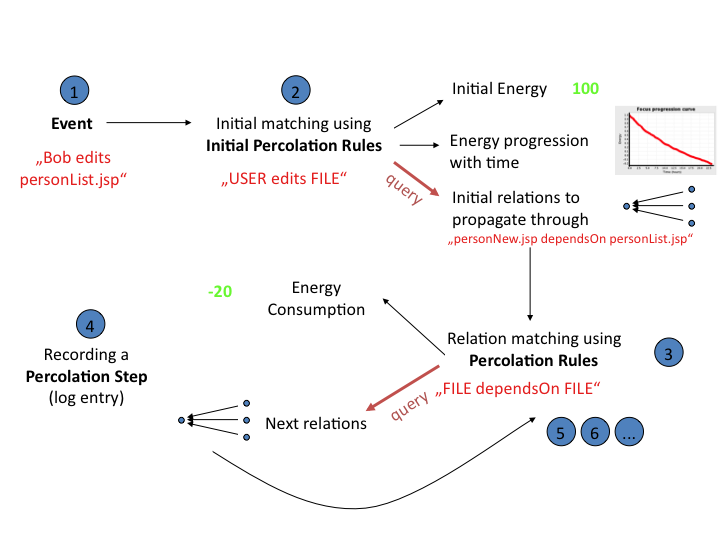
\includegraphics[width=.7\linewidth]{aether-mechanism}
  \caption{Aether mechanism}
  \label{fig:aether-mechanism}
\end{figure}

\begin{figure}[thb]
  \centering
  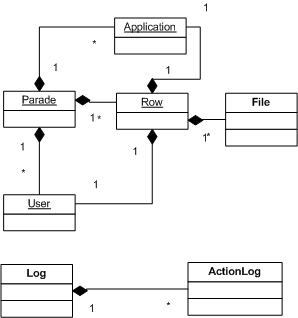
\includegraphics[width=.4\linewidth]{parade-data-model}
  \caption{Parade data model}
  \label{fig:parade-data-model}
\end{figure}

\begin{figure}[thb]
  \centering
  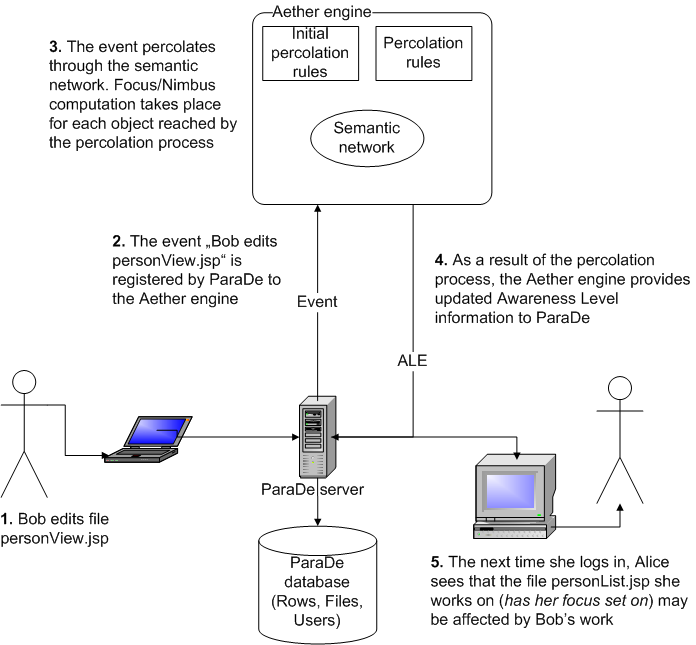
\includegraphics[width=.7\linewidth]{peroclation-example}
  \caption{Percolation example}
  \label{fig:percolation}
\end{figure}

\begin{figure}[thb]
  \centering
  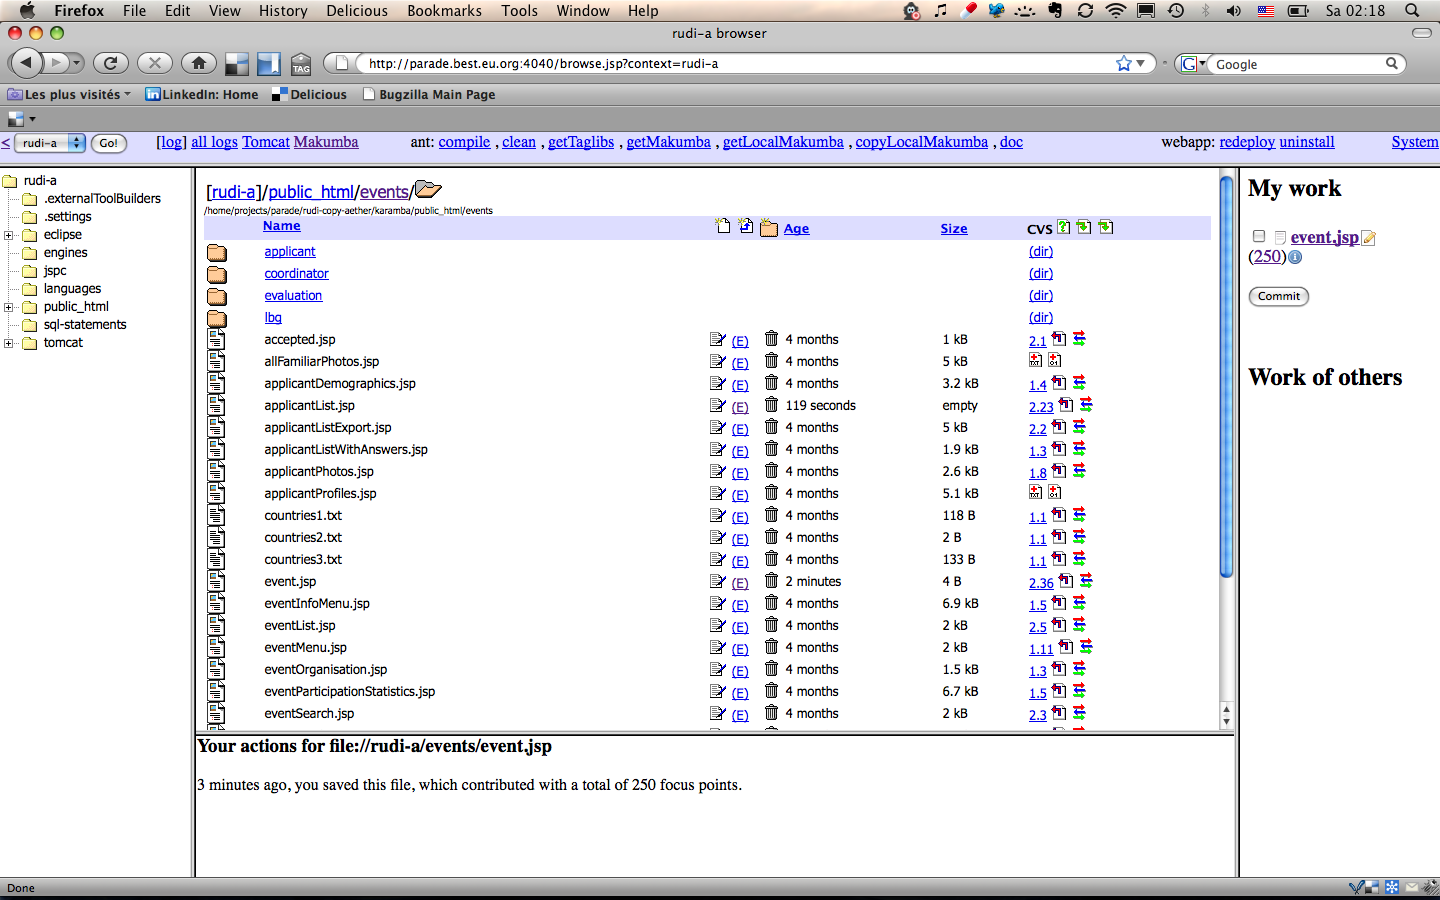
\includegraphics[width=.9\linewidth]{my-work}
  \caption{My work}
  \label{fig:my-work}
\end{figure}

\begin{figure}[thb]
  \centering
  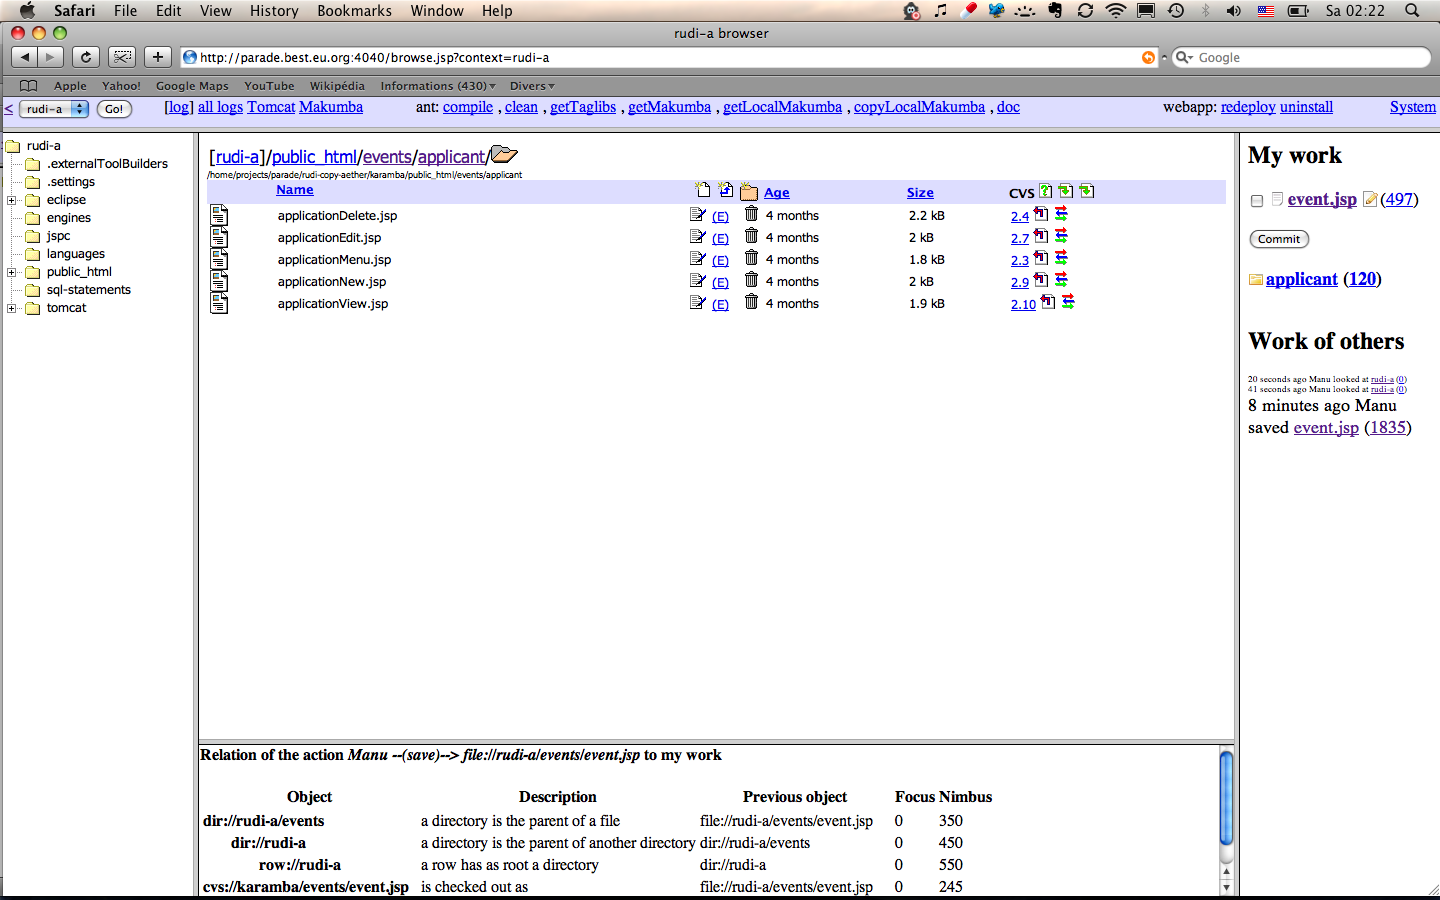
\includegraphics[width=.9\linewidth]{work-others}
  \caption{Work of others}
  \label{fig:work-others}
\end{figure}

\begin{figure}[thb]
  \centering
  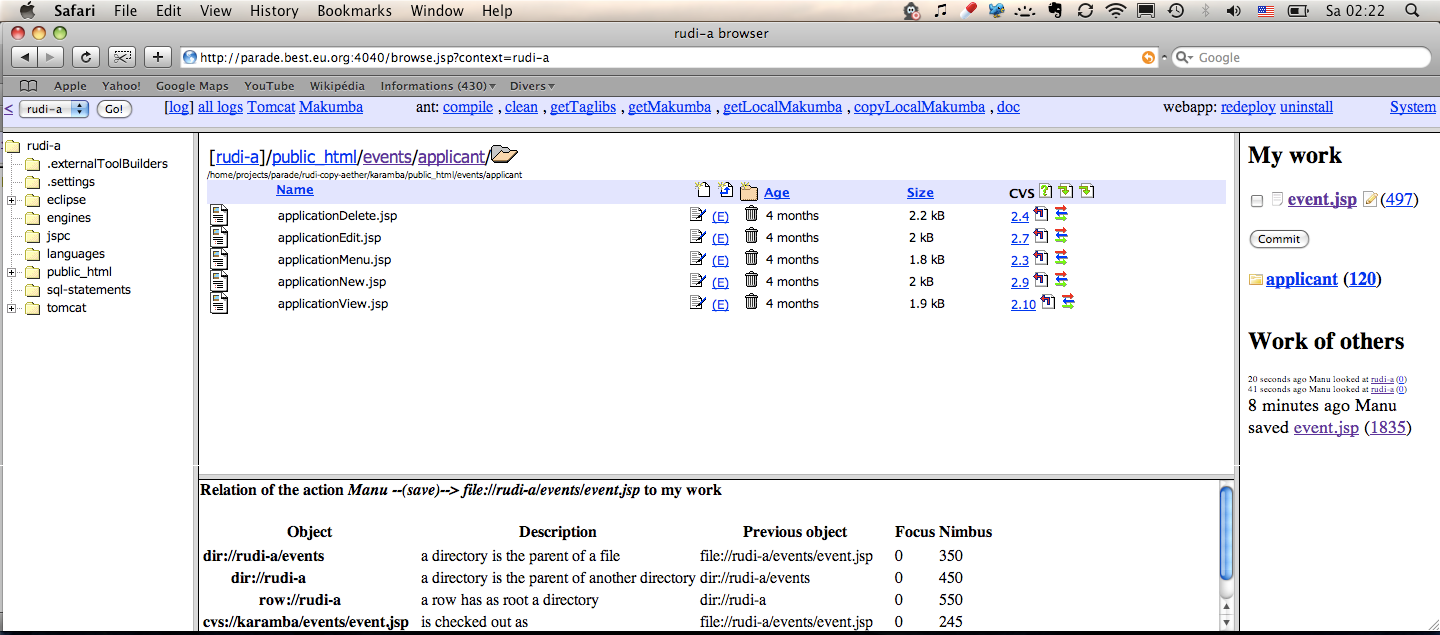
\includegraphics[width=.98\linewidth]{work-others-cropped}
  \caption{Work of others}
  \label{fig:work-others-cropped}
\end{figure}



\section*{Acknowledgments} 

{\footnotesize Acknowledgment. }



\bibliography{ecscw09-aether}
\bibliographystyle{ecscw2007}  

\end{document}

% Local Variables:
% TeX-master: t
% End:
